% CS670 - Reinforcement Learning
% Puddle World Programming Assignment
% Gabriel Dulac-Arnold <gabe@squirrelsoup.net>
% Johannes H. Jensen <johannj@stud.ntnu.no>
\documentclass[a4paper]{article}
%\usepackage{multicol}
\usepackage{graphicx}
\usepackage[top=2cm,nohead,nofoot]{geometry}
\usepackage{subfig}



\graphicspath{{../experiments/graphs/}}

\author{Gabriel Dulac-Arnold $<$gabe@squirrelsoup.net$>$ (CS09F004) \\
Johannes H. Jensen $<$johannj@stud.ntnu.no$>$ (CS09F005)}
\title{CS670 - Reinforcement Learning \\
\emph{Puddle World Programming Assignment}}

\begin{document}
\setlength{\parskip}{2ex}
\maketitle

\section{Q-Learning and Sarsa}

Q-Learning and Sarsa were both trained using a constant exploring probability 
$\epsilon = 0.1$ and learning rate $\alpha = 0.1$ over 10 000 episodes, averaged
over 50 runs.

\subsection{Goal A}

Goal A gives rapid convergence and pretty clear policies.  We notice that the policy
generated by SARSA seems a bit less chaotic than Q-learning, but we attribute this difference
to chance.

\begin{figure}[htbp!]
\center
\includegraphics[scale=0.75]{A/steps.png}
\caption{Average number of steps to reach goal}
\end{figure}

\begin{figure}[htbp!]
\center
\includegraphics[scale=0.75]{A/returns.png}
\caption{Average reward per episode}
\end{figure}

\begin{figure}[htbp!]
\center
\includegraphics[scale=0.75]{A/Q-Learning-policy.png}
\caption{Policy learned by Q-Learning}
\end{figure}

\begin{figure}[htbp!]
\center
\includegraphics[scale=0.75]{A/SARSA-policy.png}
\caption{Policy learned by Sarsa}
\end{figure}

\newpage
\subsection{Goal B}

Here we see similar results as those with goal A.  There is a very minor peak in average reward,
that seems to decrease slightly as the episodes go on.  We have no clear hypothesis for why this is
hapenning, although it could have something to do with our choice of constant $\epsilon$ for the $\epsilon$
-greedy search.

\begin{figure}[htbp!]
\center
\includegraphics[scale=0.75]{B/steps.png}
\caption{Average number of steps to reach goal}
\end{figure}

\begin{figure}[htbp!]
\center
\includegraphics[scale=0.75]{B/returns.png}
\caption{Average reward per episode}
\end{figure}

\begin{figure}[htbp!]
\center
\includegraphics[scale=0.75]{B/Q-Learning-policy.png}
\caption{Policy learned by Q-Learning}
\end{figure}

\begin{figure}[htbp!]
\center
\includegraphics[scale=0.75]{B/SARSA-policy.png}
\caption{Policy learned by Sarsa}
\end{figure}


\newpage
\subsection{Goal C}
Both SARSA and Q-Learning continue to perform well even with this more difficult goal.
The only big difference with this run is that returns peak after about 1000 episodes and
then decrease quite visibly.  Once again there is no clear cause, and our hypotheses are the
same as mentioned in goal B.

\begin{figure}[htbp!]
\center
\includegraphics[scale=0.75]{C/steps.png}
\caption{Average number of steps to reach goal}
\end{figure}

\begin{figure}[htbp!]
\center
\includegraphics[scale=0.75]{C/returns.png}
\caption{Average reward per episode}
\end{figure}

\begin{figure}[htbp!]
\center
\includegraphics[scale=0.75]{C/Q-Learning-policy.png}
\caption{Policy learned by Q-Learning}
\end{figure}

\begin{figure}[htbp!]
\center
\includegraphics[scale=0.75]{C/SARSA-policy.png}
\caption{Policy learned by Sarsa}
\end{figure}

\section{Policy Gradient}

Policy Gradient was run on an environment with deterministic actions using 
learning rate $\alpha = 0.005$ and initial temperature $\tau = 500$, which decreased to
$\tau = 1$ by the 300th episode.  The graphs are averaged over 30 runs. This method only converged for Goal A.

\begin{figure}[htbp!]
\center
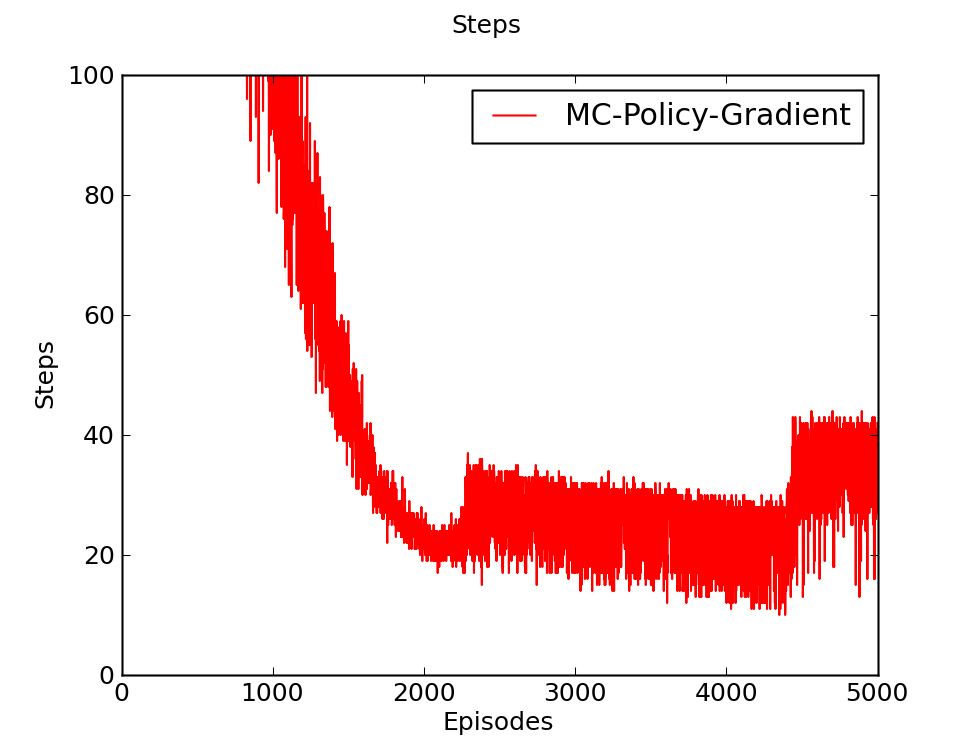
\includegraphics[scale=0.75]{A/pg-steps.png}
\caption{Average number of steps to reach goal}
\end{figure}

We notice here that we seem to attain an optimal number of steps after 2000 episodes,
and then the number of steps bumps up twice.  This would be worrying except that it seems
the longer policies give better returns, as we can see in figure 14.  Only after 4500 episodes
or so are we consistently getting a reward of 8.

\begin{figure}[htbp!]
\center
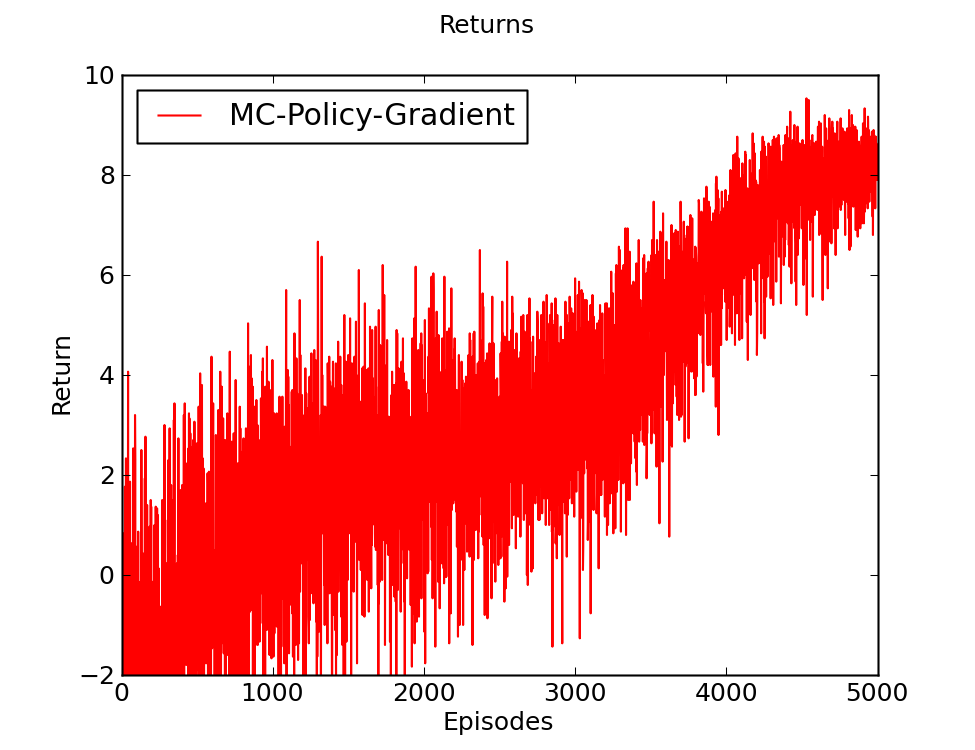
\includegraphics[scale=0.75]{A/pg-returns.png}
\caption{Average reward per episode}
\end{figure}
\begin{figure}[htbp!]
\center
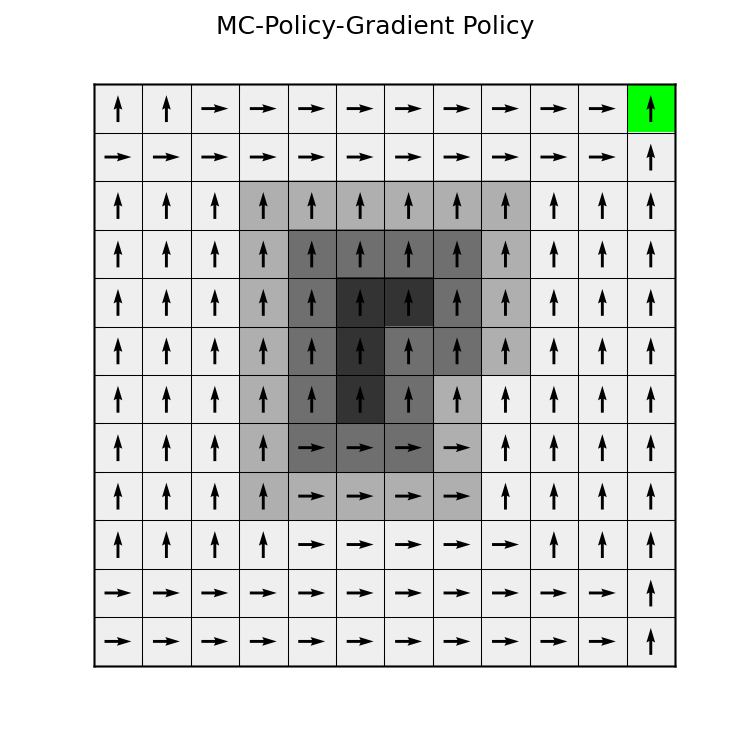
\includegraphics[scale=0.75]{A/MC-Policy-Gradient-policy.png}
\caption{Policy learned by MC Policy Gradient}
\end{figure}
\newpage
The uniformity of this policy is characteristic of a policy gradient approach.  
Even inside the puddle, areas which we would have most likely explored less, we can see
that the policy is sensible.  This is carried over from the experience of the agent in 
the zones around the puddle and is one of the clear advantages of policy gradient.
\end{document}
